%FOR PDFLATEX USE ONLY
\documentclass[a4paper,12pt]{article}

\usepackage{amssymb,amsmath} %math symbols

\usepackage[margin=2cm]{geometry} %paper geometry

\usepackage[T1, T2A]{fontenc}

\usepackage[utf8]{inputenc} %allows unicode (including russian) source file
\usepackage[russian]{babel} %docment in russian-style
\usepackage[utf8]{inputenc}
%\usepackage[unicode]{hyperref} %links inside of the text
\usepackage[pdftex]{graphicx} %includegraphics pictures
\usepackage{cmlgc} %bold text

\usepackage{array} %arrays

%\usepackage{wrapfig}
%\usepackage{array}
%\usepackage{lipsum}
%\usepackage{esvect}
%\usepackage{hyperref}

\usepackage{amsmath}
\usepackage{amssymb}
\usepackage{mathtools}
\usepackage{mathtext}

\usepackage{subfig}
%\usepackage{calc}
%\usepackage{pgfplots,tikz,circuitikz}
%\usepackage{tkz-euclide}
\usepackage{booktabs}
\usepackage{multirow}

\usepackage{wrapfig}

\renewcommand{\AA}{\ensuremath{\mathring{A}}}

\begin{document}

\begin{center}
  \LARGE{Работа 4.2.2}\\[0.2cm]
  \LARGE{Интерферометр Жамена}\\[0.2cm]
  \large{Малиновский Владимир}\\[0.2cm]
  \normalsize{\texttt{galqiwi@galqiwi.ru}}
\end{center}

\textbf{Цель работы}: ознакомление с техникой интерференционных измерений показателей преломления газов с помощью интерферометра Жамена.

\textbf{В работе используются}: интерферометр Жамена; газовая кювета; осветитель; зрительная труба; сильфон; баллон с углекислым газом; манометр; краны.

\section*{Описание работы}
Интерферометр Жамена позволяет посчитать разность хода лучей в двух газовых кюветах, путем измерения количества полос $m$, на которое сместится интерференционная картина при изменении макропараметров системы (таких, как давление или состав газа)
\[\Delta = m \lambda.\]
Поскольку разность хода и коэффициент преломления $n$ напрямую связаны, из полученных данных можно получить изменение $n$
\[\delta n = \frac{\Delta}{l} = \frac{m \lambda}{l},\]
где $l$ -- длина газовой кюветы.

\begin{center}
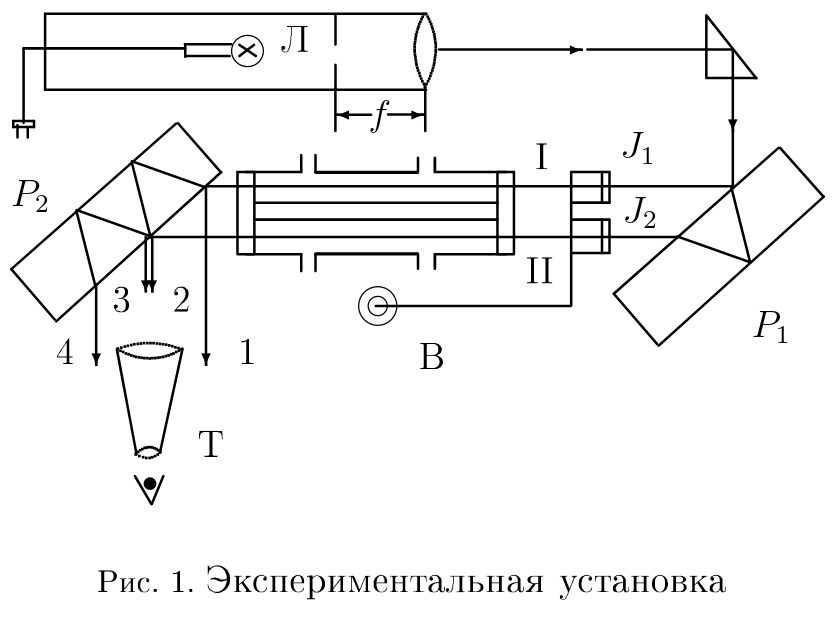
\includegraphics[width=0.60\textwidth]{0.png}
\end{center}

\section*{Результаты и измерения}
\subsection*{1-5 Юстировка}
Отъюстируем интерферометр, следуя инструкциям.
\subsection*{6-8 Калибровка}
На установке имеется микрометрический винт, поворачивая который можно добиться дополнительной разности хода между лучами. Измерим зависимость $m$ -- количество полос, на которое сдвигается интерференционная картина, в зависимости от $z$ -- показаний микрометрического винта.

\begin{center}
\begin{tabular}{|l|l|l|l|l|l|l|l|l|l|l|l|}
\hline
$z,\,\text{мм}$ & 12.87 & 13.06 & 13.27 & 13.52 & 13.74 & 13.96 & 14.23 & 14.44 & 14.68 & 14.93 & 15.18 \\ \hline
$n$             & -11   & -10   & -9    & -8    & -7    & -6    & -5    & -4    & -3    & -2    & -1    \\ \hline
\end{tabular}\\~\\~\\

\begin{tabular}{|l|l|l|l|l|l|l|l|l|l|l|l|}
\hline
$z,\,\text{мм}$ & 15.45 & 15.75 & 16.03 & 16.32 & 16.62 & 16.97 & 17.29 & 17.67 & 18.01 & 18.38 & 18.83 \\ \hline
$n$             & 0     & 1     & 2     & 3     & 4     & 5     & 6     & 7     & 8     & 9     & 10    \\ \hline
\end{tabular}\\~\\~\\

\begin{tabular}{|l|l|l|l|l|l|l|}
\hline
$z,\,\text{мм}$ & 19.17 & 19.68 & 20.12 & 20.71 & 21.24 & 21.9 \\ \hline
$n$             & 11    & 12    & 13    & 14    & 15    & 16   \\ \hline
\end{tabular}\\~\\~\\

$\Delta z = 0.01\,\text{мм}$

\end{center}

\begin{center}
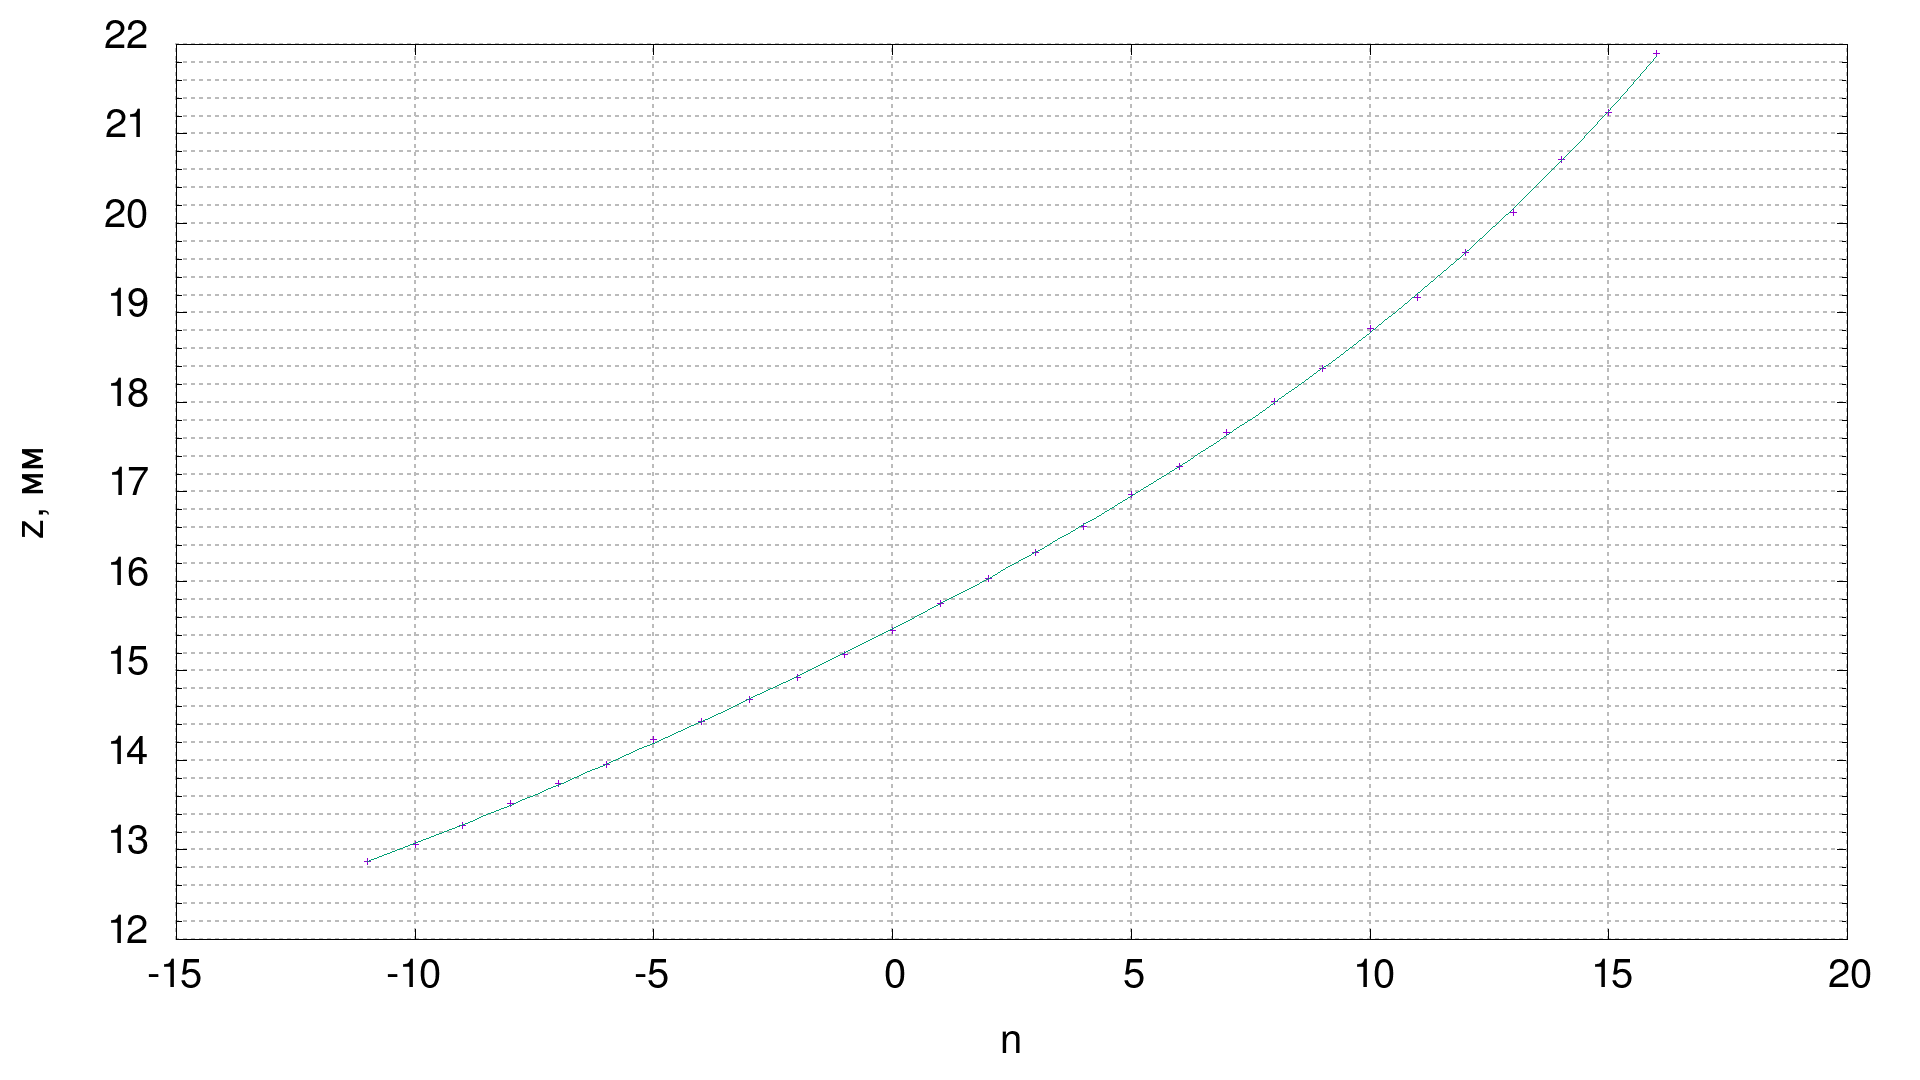
\includegraphics[width=0.90\textwidth]{1.png}
\end{center}

После того, как мы измерили калибровочную кривую, мы можем точно определять сдвиг интерференционной картины по показанию микрометрического винта.

\newpage

\subsection*{9-10 Зависимость $\delta n$ от $P$ для воздуха}

Измерим разность хода через смещение полос от давления $P$ воздуха. Во время измерений смещение нулевой полосы $\Delta_0$ при нулевом давлении заметно менялась, из-за чего для каждого значения давления мы записывали не только показания микрометрового винта в конце измерений $z_0$, но и в конце $z_1$.

\begin{center}
\begin{tabular}{|c|c|c|c|c|c|}\hline
$\Delta P\text{, кПа}$&$z_0\text{, \text{мм}}$&$\Delta_0\text{, мкм}$&$z_1\text{, \text{мм}}$&$\Delta_1\text{, мкм}$&$\Delta\text{, мкм}$\\\hline
$9.0$&$16.95$&$3.2$&$18.20$&$5.5$&$2.3$\\\hline
$6.0$&$17.40$&$4.1$&$18.25$&$5.6$&$1.5$\\\hline
$4.0$&$17.10$&$3.5$&$17.65$&$4.6$&$1.0$\\\hline
$2.0$&$18.04$&$5.3$&$18.35$&$5.8$&$0.5$\\\hline
$0.0$&$17.65$&$4.6$&$17.65$&$4.6$&$0.0$\\\hline
$-2.5$&$19.03$&$6.9$&$18.63$&$6.3$&$-0.6$\\\hline
$-5.0$&$19.19$&$7.1$&$18.48$&$6.0$&$-1.1$\\\hline
$-7.5$&$19.82$&$8.0$&$18.53$&$6.1$&$-1.9$\\\hline
$-10.0$&$20.21$&$8.5$&$18.53$&$6.1$&$-2.4$\\\hline
\end{tabular}\\~\\
$\Delta (\Delta P)=0.5\,\text{кПа}, \Delta z_0=\Delta z_1=0.01\,\text{\text{мм}}, \Delta (\Delta_0)=\Delta (\Delta_1)=0.3\,\text{мкм}, \Delta (\Delta)=0.4\,\text{мкм}$
\end{center}



\begin{center}
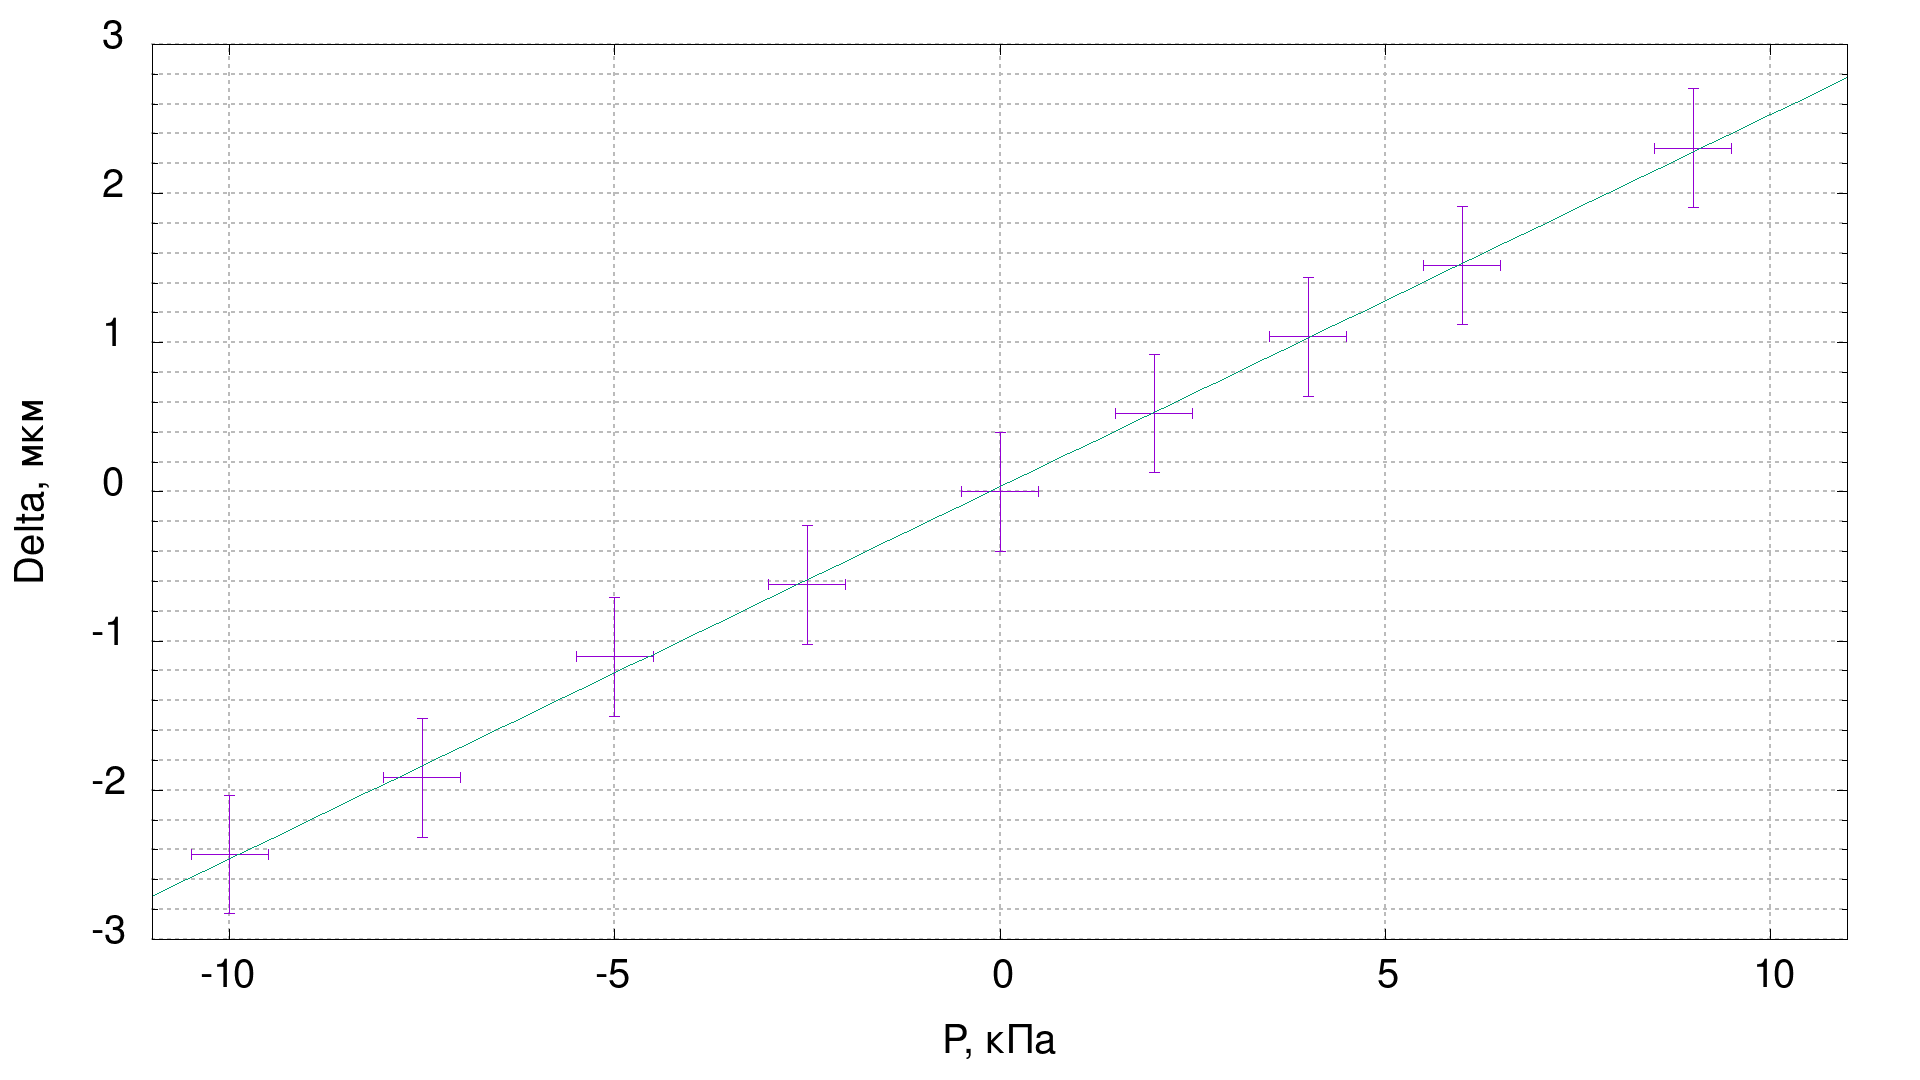
\includegraphics[width=0.90\textwidth]{2.png}
\end{center}

Известно, что
\[\Delta = \frac{2\pi\alpha l}{kT}\Delta P.\]
Из графика можно найти, что
\[\frac{\Delta}{\Delta P} = (0.25 \pm 0.04)\frac{\text{нм}}{\text{Па}}.\]
Если подставить условия ($T=298.45\,\text{К}, l=0.1\,\text{м}$), то можно получить поляризуемость молекулы азота
\[\alpha = (1.7\pm0.30) \cdot 10^{-30}\,\text{м}^3.\]

Согласно электронному справочнику на chemport.ru, поляризуемость молекулы азота равна
\[\alpha_0 = 1.734 \cdot 10^{-30}\,\text{м}^3\]
что соответствует нашим наблюдениям.

Если считать молекулу азота малым металическим шариком, то ее поляризацию можно выразить через радиус как
\[\alpha = 4 \pi r^3,\]
что дает нам значение радиуса
\[r \approx 0.5 \AA.\]
Это значение совпадает в порядке с табличным (взятым с ido.tsu.ru)
\[r \approx 0.15 \AA.\]
\subsection{11-14 Сравнение показателей преломления воздуха и углекислого газа при атмосферном давлении}

Измерим разность $\delta n$ от времени для смеси углекислого газа с воздухом.

\begin{center}
\begin{tabular}{|c|c|c|}\hline
$t\text{, min}$&$z\text{, mm}$&$\delta n, 10^{-5}$\\\hline
$0$&$17.96$&$5.1$\\\hline
$1.0$&$17.91$&$5.0$\\\hline
$2.0$&$17.80$&$4.8$\\\hline
$3.0$&$17.75$&$4.8$\\\hline
$4.0$&$17.72$&$4.7$\\\hline
$5.0$&$17.67$&$4.6$\\\hline
$6.0$&$17.68$&$4.6$\\\hline
$7.0$&$17.63$&$4.5$\\\hline
$8.0$&$17.59$&$4.5$\\\hline
$9.0$&$17.54$&$4.4$\\\hline
$10.0$&$17.53$&$4.4$\\\hline
$11.0$&$17.49$&$4.3$\\\hline
$12.0$&$17.45$&$4.2$\\\hline
$13.0$&$17.41$&$4.1$\\\hline
$14.0$&$17.34$&$4.0$\\\hline
$15.0$&$17.35$&$4.0$\\\hline
\end{tabular}\\~\\
$\Delta z=0.01\,\text{mm}, \Delta \delta n=0.4\cdot10^{-5}$
\end{center}


\begin{center}
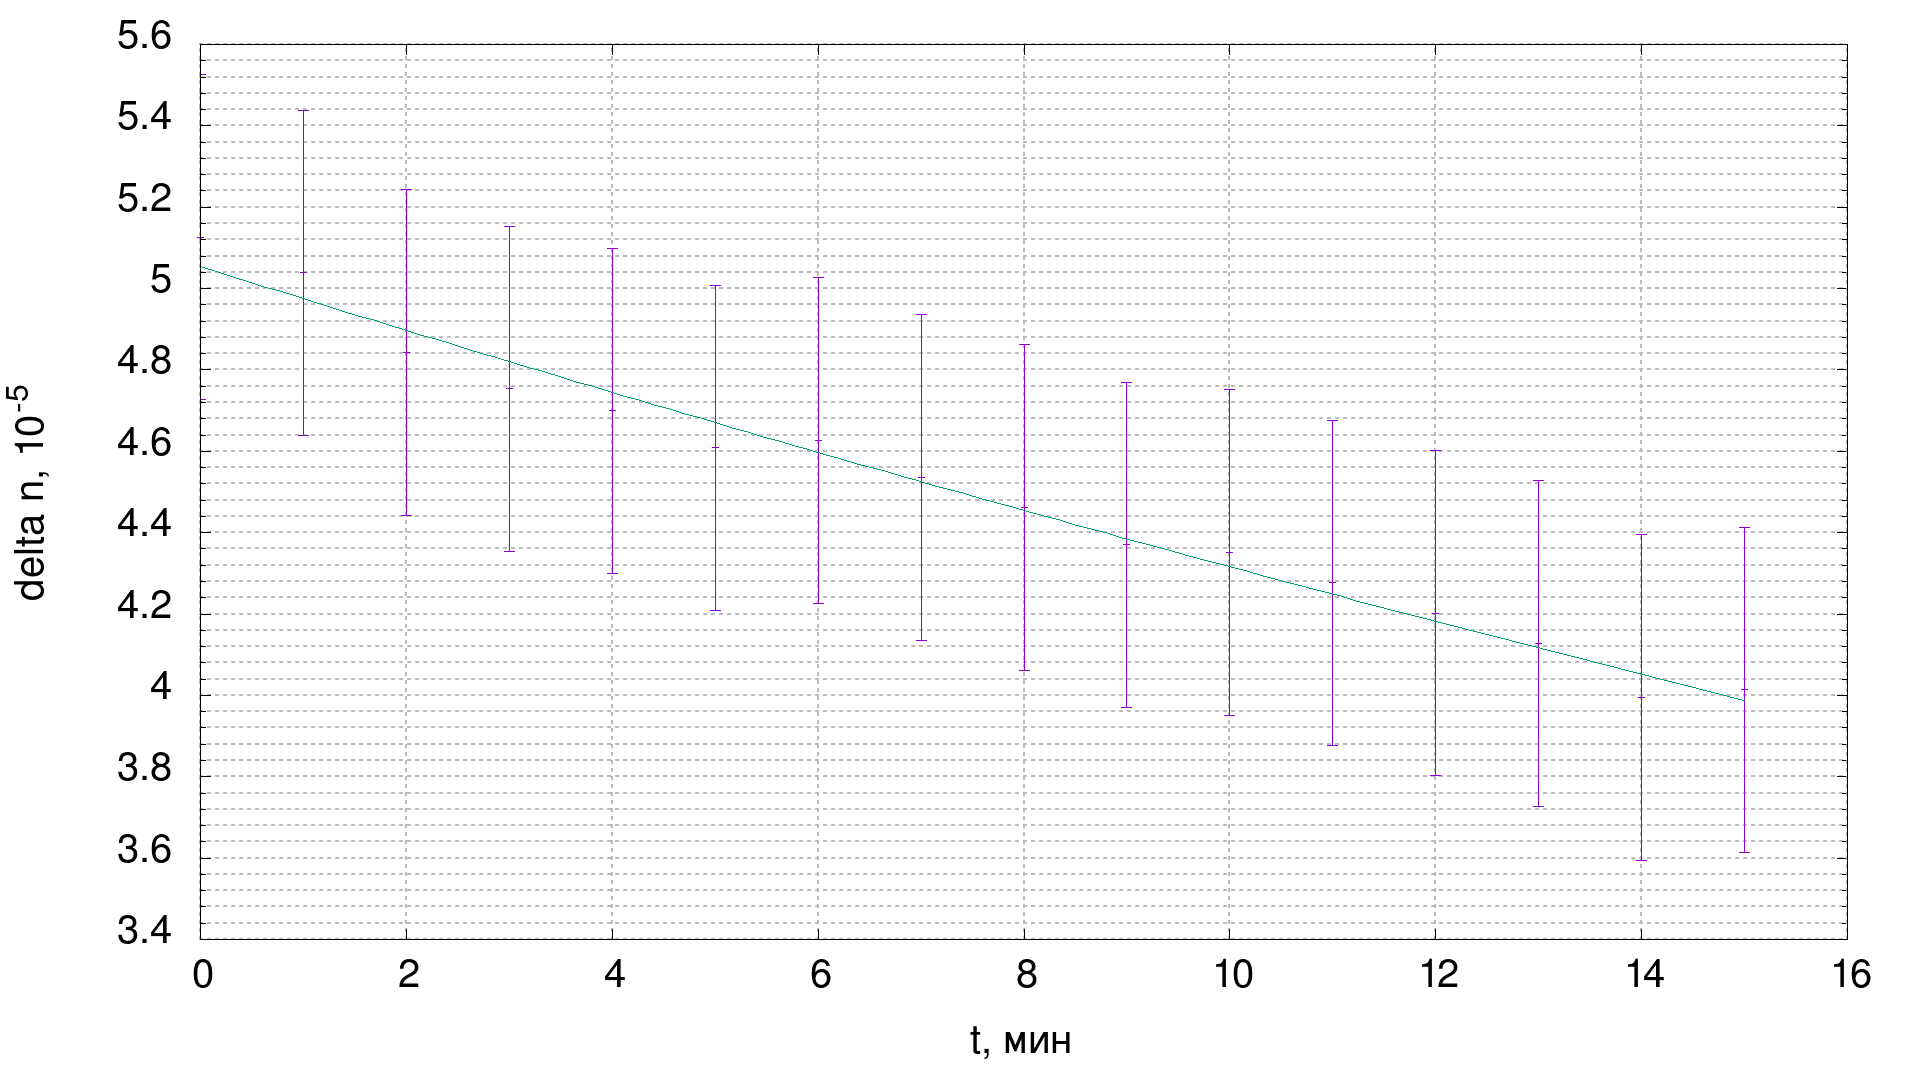
\includegraphics[width=0.90\textwidth]{3.png}
\end{center}

Как видно, происходит утечка углекислого газа.

\subsection{оценка интервала $\Delta$}
Во время калибровки мы происследовали весь достижимый диапазон значений $n$. При выходе за него, полосы начинали либо накладываться друг на друга, либо становились настолько тусклыми, что их нельзя больше измерить. Это облегчает нам оценку $\Delta n_{max}$
\[\Delta n_{max} = 7.2 \cdot 10^{-5}.\]
Минимальное значение $\Delta$, которое мы можем измерить достигается при отклонении микрометрового винта на $10$ микрометров.
\[\Delta n_{min} = 1.9 \cdot 10^{-7}.\]

\section*{Вывод}
Мы научились исследовать макро и микропараметры системы через эффекты волновой оптики. С помощью интерферометра Жамена мы получили зависимость коэффициента преломления от давления у воздуха и вывели численные значения для молекул азота
\[r \approx 0.5 \AA,\]
\[\alpha = (1.7\pm0.30) \cdot 10^{-30}\,\text{м}^3.\]
Эти численные значения совпали с табличными данными
\[r \approx 0.15 \AA,\]
\[\alpha_0 = 1.734 \cdot 10^{-30}\,\text{м}^3.\]
Также мы получили свидетельство наличия протечки углекислого газа через изменение показателя преломления.

\end{document}








\lipsum[1-4]
\begin{wrapfigure}{R}{5cm}
\centering
\includegraphics[width=0.20\textwidth]{rd.png}
\caption{1}
\end{wrapfigure}
\lipsum[1-6]


\begin{figure}[h]
\begin{center}$
\begin{array}{cccc}
\includegraphics[width=0.20\textwidth]{rd.png}&
\includegraphics[width=0.20\textwidth]{rd.png}&
\includegraphics[width=0.20\textwidth]{rd.png}&
\includegraphics[width=0.20\textwidth]{rd.png}\\
(1) & (2) & (3) & (4)
\end{array}$
\end{center}
\end{figure}
